
\begin{enumerate}
	
\item The dual problem is
\[
\max_{y \in \mathbb{R}^2} \quad y_1 + 2y_2
\]
subject to
\begin{align*}
-2y_1+y_2 &\leq 2 \qquad  (x_1),\\
-y_1+2y_2 &\leq 7  \qquad  (x_2),\\
y_1 &\leq 3  \qquad  (x_3),\\
y_1,y_2&\geq 0.
\end{align*}	

	\begin{center}
		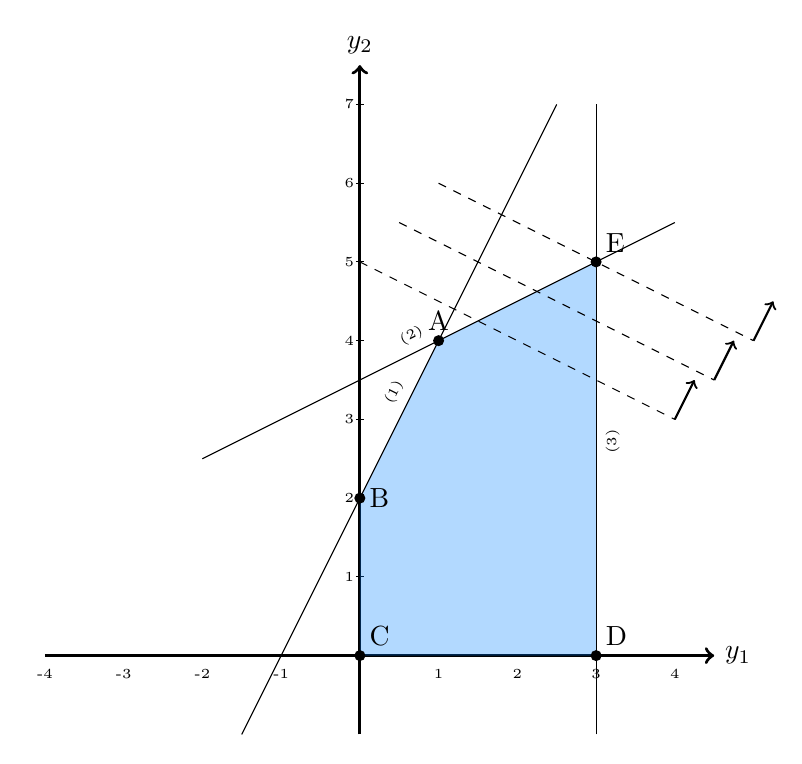
\begin{tikzpicture}
		%\draw[gray!50, thin, step=0.5] (0,0) grid (8,8);
		\draw[very thick,->] (0,1) coordinate(x1) -- (8.5,1) coordinate(x2) node[right] {$y_1$};
		\draw[very thick,->] (4,0) coordinate(y1) -- (4,8.5) coordinate(y2) node[above] {$y_2$};
		\foreach \x in {-4,...,-1} \draw (\x+4,0.95) -- (\x+4,0.95) node[below] {\tiny\x};
		\foreach \x in {1,...,4} \draw (\x+4,0.95) -- (\x+4,0.95) node[below] {\tiny\x};
		\foreach \y in {1,...,7} \draw (3.95,\y+1) -- (4.05,\y+1) node[left] {\tiny\y};
		\fill[blue!50!cyan,opacity=0.3] (4,1) -- (4,3) -- (5,5) -- (7,6) -- (7,1) -- cycle;    
		\draw (2.5,0) coordinate (a1) -- node[above right,sloped] {\tiny $(1)$} (6.5,8) coordinate (a2);
		\draw (2,3.5) coordinate (b1) -- node[above left,sloped] {\tiny $(2)$} (8,6.5) coordinate (b2);
		\draw (7,0) coordinate (c1) -- node[below left,sloped] {\tiny $(3)$} (7,8) coordinate (c2);
		\coordinate (v1) at (intersection of a1--a2 and b1--b2);
		\coordinate (v2) at (intersection of a1--a2 and y1--y2);
		\coordinate (v3) at (intersection of x1--x2 and y1--y2);
		\coordinate (v4) at (intersection of x1--x2 and c1--c2);
		\coordinate (v5) at (intersection of b1--b2 and c1--c2);
		\fill[black] (v1) node[above] {A} circle (2pt);
		\fill[black] (v2) node[right] {B} circle (2pt);
		\fill[black] (v3) node[above right] {C} circle (2pt);
		\fill[black] (v4) node[above right] {D} circle (2pt);
		\fill[black] (v5) node[above right] {E} circle (2pt);
		
		\draw[dashed] (4,6) coordinate (b1) -- (8,4) coordinate (b2);
		\draw[dashed] (4.5,6.5) coordinate (b1) -- (8.5,4.5) coordinate (b2);
		\draw[dashed] (5,7) coordinate (b1) -- (9,5) coordinate (b2);
		
		\draw[->,thick] (8,4)--(8.25,4.5);
		\draw[->,thick] (8.5,4.5)--(8.75,5);
		\draw[->,thick] (9,5)--(9.25,5.5);
		\end{tikzpicture}
	\end{center}

The graphical solution to the dual problem is given in the above figure. The optimal solution to the dual denoted by point $E$ is
\[
\rvect{y^*_1 \\ y^*_2}= \rvect{3 \\ 5},
\]
and the optimal objective function value is $13$.


\item The complementarity slackness conditions are stated as follows. 
Consider the primal linear problem
\[
\min_{x \in \mathbb{R}^n} c^{T}x
\]
subject to
\[
Ax = b,
\]
\[
x \geq 0,
\]
where $A \in \mathbb{R}^{m x n}$, $b \in \mathbb{R}^n$, $c \in \mathbb{R}^n$, and the dual problem
\[
\max_{\lambda \in \mathbb{R}^m} \lambda^{T}b
\]
subject to
\[
A^T \lambda \leq c .
\]
Consider $x^*$ primal feasible and $\lambda^*$ dual feasible. $x^*$ is optimal for the primal and $\lambda^*$ is optimal for the dual if and only if
\[
(c_i - \sum_{j=1}^{m} a_{ji} \lambda_j^*) x_i^* = 0,  \quad  i=1,...,n.
\]

These conditions mean that if a primal variable is non zero, then the
corresponding dual constraint must be active, and if the dual
constraint is inactive, then the primal variable must be equal to
$0$. 

In order to utilize this theorem, we first write the standard form of the original problem as follows:

%. We change the variables $x_1$, $x_2$, and $x_3$ and include $x_1'$, $x_2'$, and $x_3'$ to have non negative decision variables.
%
%\[
%x_1' = -x_1 , \quad
%x_2' = -x_2 , \quad
%x_3' = -x_3 , \quad
%\]
%
%Then the standard form becomes

\[
\min_{x \in \mathbb{R}^5} \quad 2x_1 + 7x_2+ 3x_3
\]
subject to
\begin{align*}
-2x_1-x_2+x_3-x_4 &= 1 \quad (y_1), \\
x_1+2x_2-x_5 &= 2 \quad (y_2), \\
x_1,x_2,x_3,x_4,x_5 &\geq 0.
\end{align*}

The dual of the standard form is then

\[
\max_{y \in \mathbb{R}^2} \quad y_1 + 2y_2
\]
subject to
\begin{align*}
-2y_1+y_2 &\leq 2 \quad (x_1),\\
-y_1+2y_2 &\leq 7 \quad (x_2),\\
y_1 &\leq 3 \quad (x_3),\\
-y_1 &\leq 0 \quad (x_4),\\
-y_2 &\leq 0 \quad (x_5),\\
y_1,y_2& \in \mathbb{R}.
\end{align*}

%Please notice that as we made change of variables, the dual problem above is not the same with the dual we have written in the first part.

%Now, we solve the dual problem with the graphical method and find the optimal solution. From the graph, we see that the solution is
%
% \[
%\rvect{y^*_1 \\ y^*_2}= \rvect{3 \\ 5},
%\]
%
%and the optimal objective function value is $13$.

As we have solved the dual problem, we know  that  
 \[
\rvect{y^*_1 \\ y^*_2}= \rvect{3 \\ 5},
\]
and the optimal objective function value is $13$.
We then write the complementarity slackness conditions that need to be satisfied at optimality:
\begin{align*}
(c_1-(-2y_1^*+y_2^*))x_1^* &= 0, \\
(c_2-(-y_1^*+2y_2^*))x_2^* &= 0, \\
(c_3-(y_1^*))x_3^* &= 0, \\
(c_4-(-y_1^*))x_4^* &= 0, \\
(c_5-(-y_2^*))x_5^* &= 0, \\
\end{align*}
where $c^{T} = (2, 7, 3,0,0)$ and $y_1^* = 3$, $y_2^*=5$. Using this information, we get the following equalities:
 \begin{align*}
 3x_1^* &= 0, \\
0x_2^* &= 0, \\
0x_3^* &= 0, \\
 3x_4^* &= 0, \\
5x_5^* &= 0.
 \end{align*}
We deduce that $x_1^* = x_4^* = x_5^* = 0$. As $x^*$ must
be feasible, we replace
 $x_1^*, x_4^*,$ and $x_5^*$ in the constraints of the original problem:
\begin{align*}
-x^*_2+x^*_3 &= 1, \\
2x^*_2 &= 2.
\end{align*}
 Therefore, $x^*_2=1$ and $x^*_3=2$. The optimal solution to the
 primal problem is therefore $(x_1^*,x_2^*,x_3^*,x_4^*,x_5^*)=(0,1,2,0,0)$ and
 the objective function value is $13$.

\item The primal problem has $x_2$ and $x_3$ in the basis at 
  optimality, so that
  \[
  c_B = \rvect{7 \\ 3}.
  \]
The optimal basis matrix is given by
\[
B=\left(
\begin{array}{rr}
-1&1 \\ 2&0
\end{array} \right).
\]
Then,
\[
B^{T}=\left(\begin{array}{rr}
-1&2 \\ 1&0
\end{array} \right).
\]
The result is then verified as: 
\[
B^Ty^* = B^T\rvect{y^*_1 \\ y^*_2} =\left(
\begin{array}{cc}
-1&2 \\ 1&0
\end{array}
\right)\rvect{3 \\ 5}  = \rvect{7 \\ 3}   =  c_B.
\]
\end{enumerate}

